\begin{enumerate}[label=\thechapter.\arabic*,ref=\thechapter.\theenumi]
\item
For the circuit given below, choose the angular frequency $ \omega_0$ at which voltage across capacitor has maximum amplitude?
\begin{figure}[h!]
    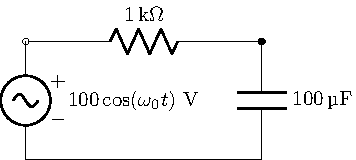
\includegraphics[width = 0.5\columnwidth]{2023/BM/16/figs/c_fig1.pdf}
    \caption{circuit }
    \centering
    \label{fig: bm_16_fig_1}
\end{figure}
\begin{enumerate}
    \item[(A)] 1000
    \item[(B)] 100
    \item[(C)] 1
    \item[(D)] 0   
\end{enumerate}
\hfill(GATE BM 2023 Question 16)\\
\pagebreak

\item In the circuit shown ,$\omega=100\pi\text{rads/s}$, R1=R2=$2.2\Omega$ and L=$7\text{mH}$. the capacitance $\text{C}$ for which $Y_{in}$ is purely real is \marco $\text{mF}$ \\
	\vspace{0.3cm}
	\begin{center}
	\begin{circuitikz} \centering \draw 
		(0,4) to[sinusoidal voltage source, l=$V_{0}$cos($\omega$t)] (0,0)
		(0,4) to[short] (4,4)
		(4,4) to[resistor, l=$R_1$ ] (4,2)
		(4,2) to[inductor, l= $\text{L} $] (4,0) to[short ] (0,0)
		(8,4)  to[short] (4,4)
		(8,4) to[resistor, l= $R_2$] (8,2) to[capacitor,l=$\text{C}$] (8,0) to (4,0)
		;
	\end{circuitikz}
	\end{center}
\hfill(GATE IN  2023 Question 46)\\
\solution
\pagebreak
\end{enumerate}
